\documentclass[11pt]{article}
\usepackage{hyperref} 
\usepackage{amsmath, amsfonts, amssymb}
\usepackage{graphicx}
\usepackage{float}
\usepackage[margin=1in]{geometry}

\parindent0px

\emergencystretch=0pt
\pretolerance=150
\tolerance=10000
\hbadness=10000
\hfuzz=0pt

\title{Investments and Derivatives Notes}
\author{Nathan Ueda}
\date{\today} 

\begin{document}
\maketitle 
\pagebreak
\tableofcontents 
\pagebreak

\section{Financial Markets}
\subsection{Assets and Securities}
\begin{itemize}
    \item An \textit{asset} is anything that has economic value. 
    \item 
\end{itemize}

\section{Modern Portfolio Theory}

\subsection{Summary}
\begin{itemize}
    \item We have some investors trying to figure out how to allocate their wealth across an 
    arbitrary portfolio of risky assets.
    \item We started with only risky investments available for this investor and came up with a
    two fund theorem that we can characterize the optimal portfolio choice of the investor, if 
    they have mean variance prefenrences.
    \item Next, we introduced a risk free asset into this portfolio.
    % TODO 
\end{itemize}

% \begin{figure}[H] 
%     \centering 
%     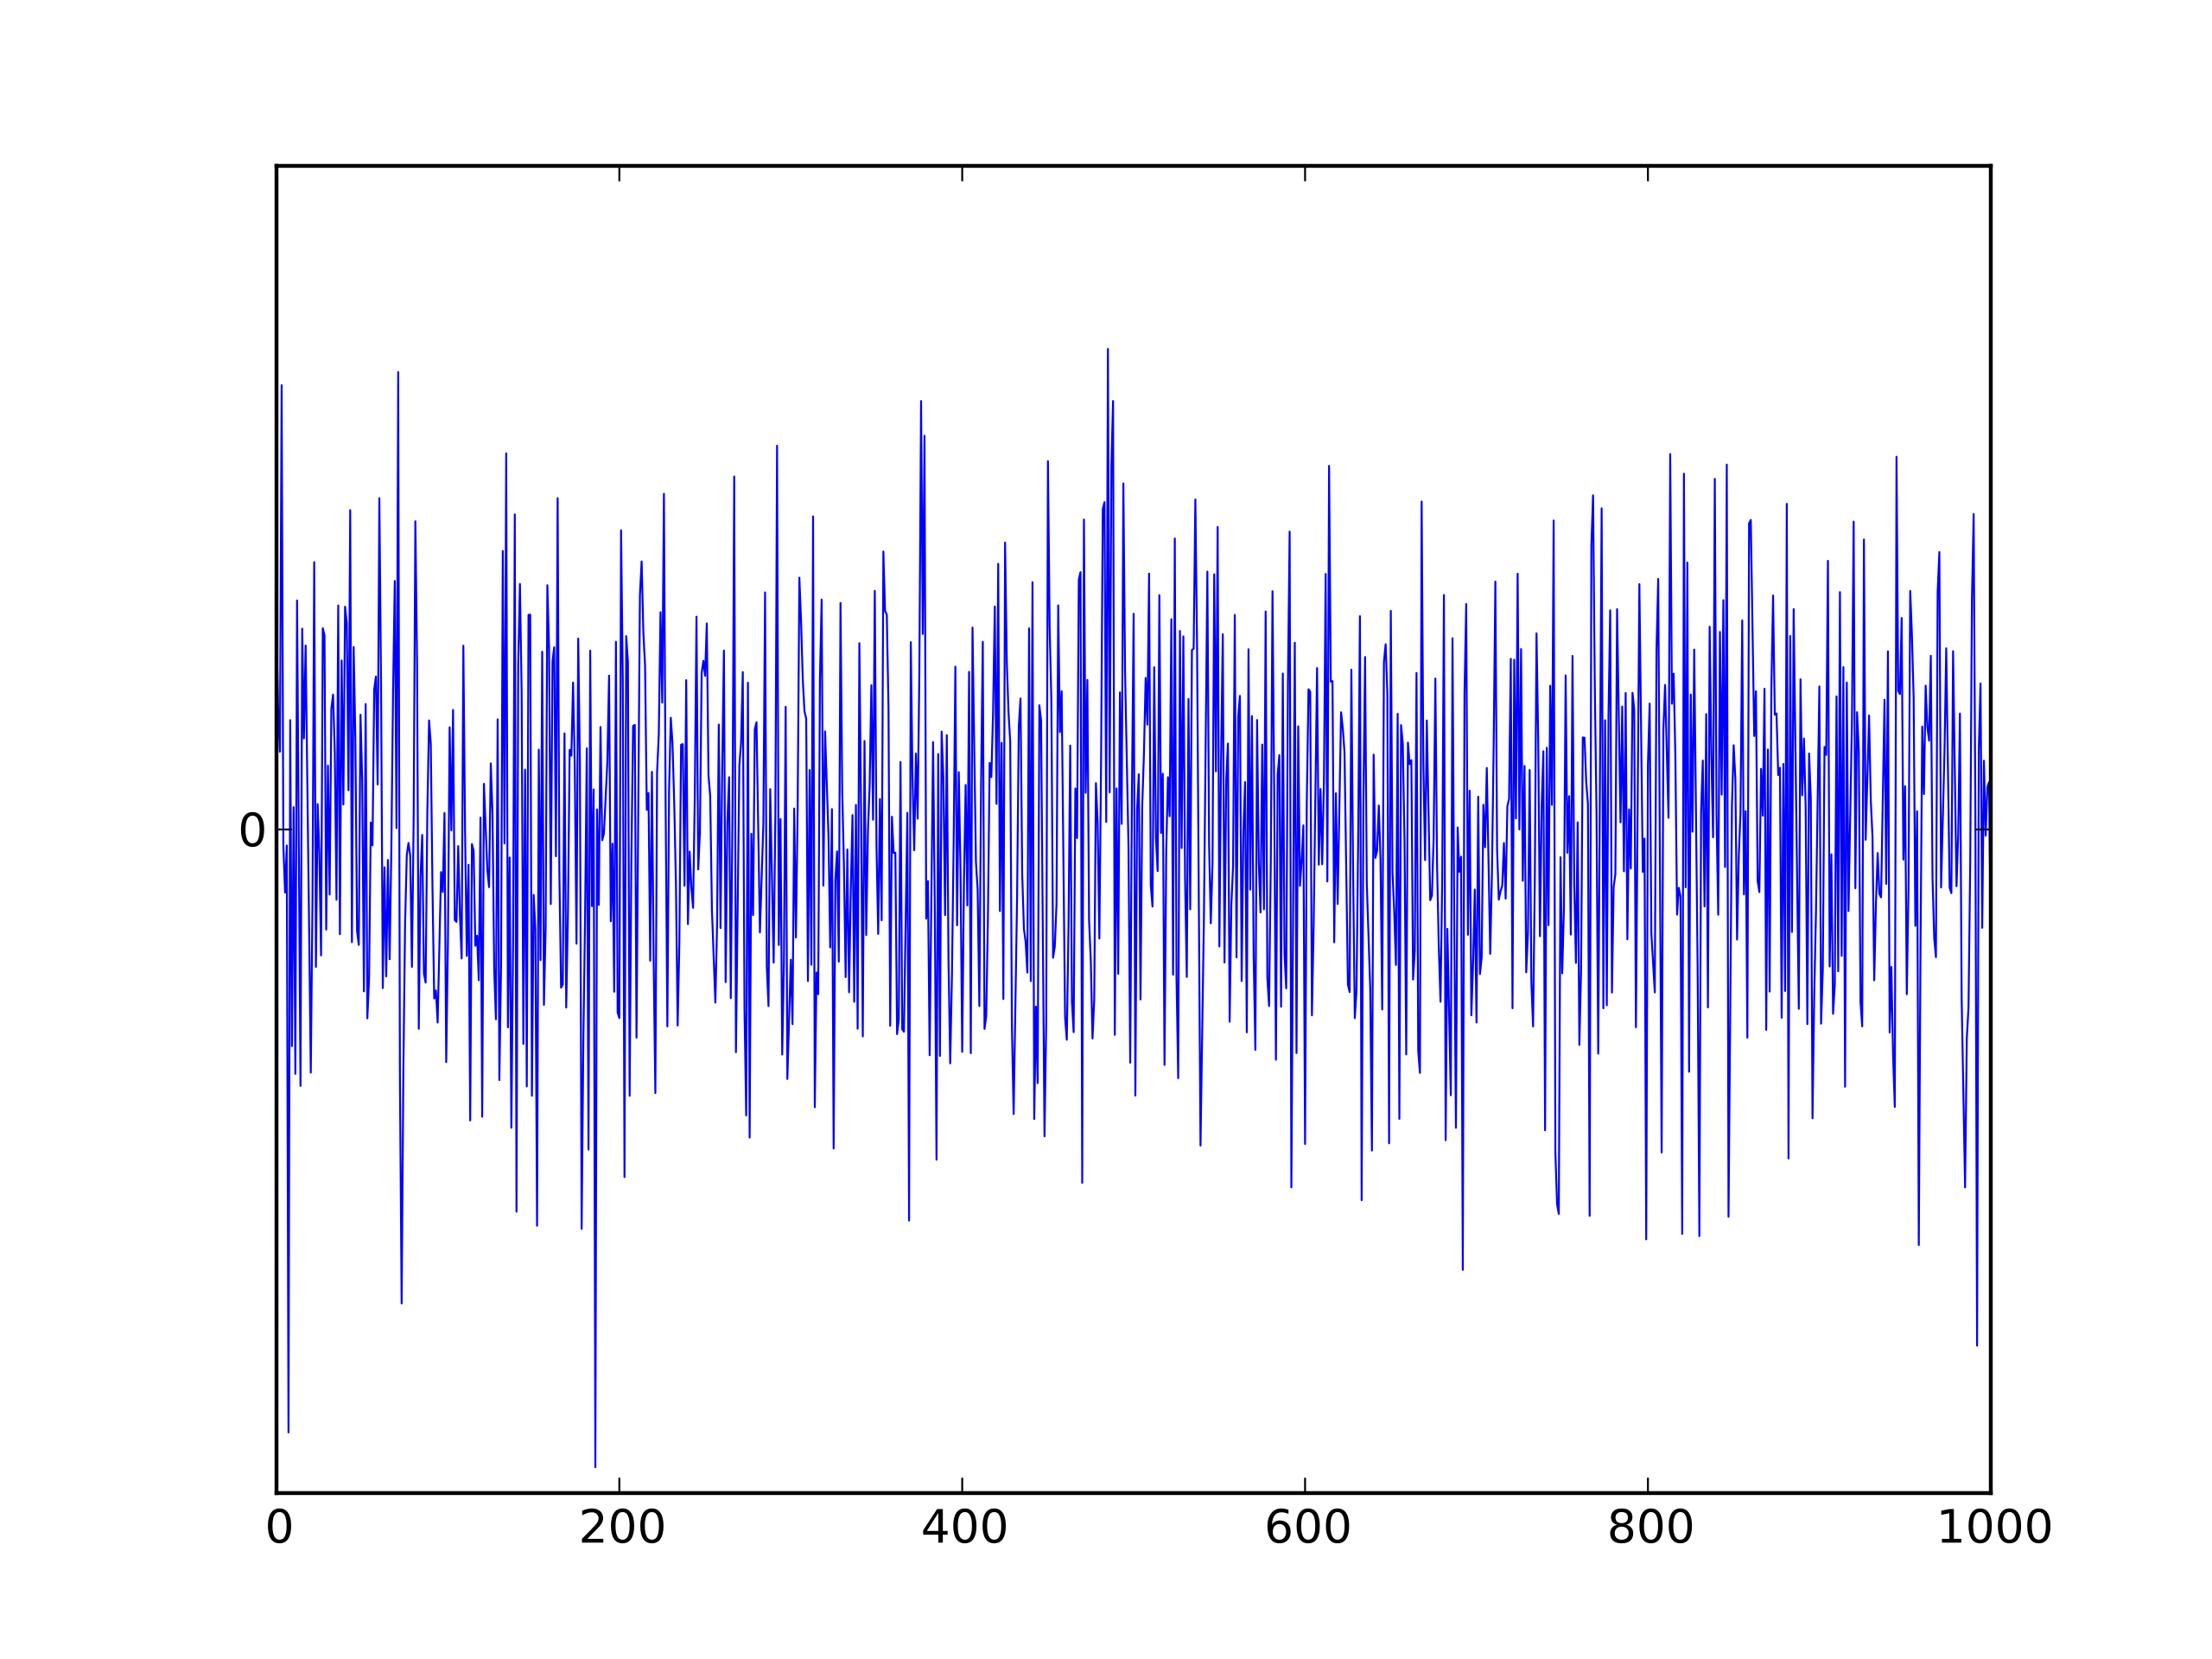
\includegraphics[width=4in]{imgs/white_noise.png}
%     \caption{White noise}
% \end{figure}

\end{document}
